\documentclass[letterpaper]{article} % DO NOT CHANGE THIS
\usepackage[submission]{aaai2027}  % DO NOT CHANGE THIS
% The serif, sans-serif, and monospaced fonts are loaded automatically by
% aaai2027.sty (newtxtext, helvet, courier). DO NOT add \usepackage{times},
% \usepackage{helvet}, \usepackage{courier}, or any other font package.
\usepackage[hyphens]{url}  % DO NOT CHANGE THIS
\usepackage{graphicx} % DO NOT CHANGE THIS
\urlstyle{rm} % DO NOT CHANGE THIS
\def\UrlFont{\rm}  % DO NOT CHANGE THIS
\usepackage{natbib}  % DO NOT CHANGE THIS AND DO NOT ADD ANY OPTIONS TO IT
\usepackage{caption} % DO NOT CHANGE THIS AND DO NOT ADD ANY OPTIONS TO IT
\frenchspacing  % DO NOT CHANGE THIS

\usepackage{booktabs}
\usepackage{algorithm}
\usepackage{algorithmic}
\pdfinfo{
/TemplateVersion (2027.1)
}
\setcounter{secnumdepth}{0}

\title{PHALCON: Discovering Intermediate Goals from Partial Success in Program Synthesis}
\author{}
\affiliations{}

\begin{document}
\maketitle

\begin{abstract}
% Write the abstract here.
\end{abstract}

\section{Introduction}

Programming by example (PBE), or inductive program synthesis (IPS),
is the combinatorial search problem of finding a function that correctly
maps given input examples to their corresponding output examples.
The search space is too large to explore exhaustively, so IPS techniques
rely on pruning infeasible regions or guiding search toward promising
regions.

Failure-driven approaches use incorrect behavior to prune the search
space. Counterexample-guided synthesis finds an input on which a candidate
fails and uses it to rule out candidates with the same failure
\citep{solarlezama2006sketching}. Success-driven approaches use successful
behavior to identify promising regions. Probe learns from partial
solutions to decide what to try next \citep{barke2020probe}. BUSTLE
learns which pieces of a program are likely to be useful, and CrossBeam
learns how to combine them. Both learn from solutions to training tasks
and reuse that guidance across tasks in the same domain
\citep{odena2021bustle,shi2022crossbeam}.

These approaches learn from complete solutions or from partial solutions
that completely solve some examples.
But search can stall before any candidate produces a correct output on
even one example. We therefore ask:
\textbf{How can a synthesizer extract explicit goals from candidates
that do not produce a correct output on any example?}

To set explicit goals, we use properties. A property
captures a detail of an output, and the goal is to match the target program on
that detail. For example, a string-length property sets the
goal of producing a string of the same length as the target, without
specifying its characters. Or consider a task that asks a program to turn
\texttt{John Doe} into \texttt{J Doe}. A candidate that returns
\texttt{J} gets the initial right but leaves out the surname. The
property \(\mathrm{first}(y)\) takes the first character of an output \(y\) and
returns \texttt{J} for both outputs. Using this property as a goal
guides the next search toward programs whose outputs start with the
expected initial.

The first character is an obvious choice in this example. But for a new
task, the synthesizer has to decide which property captures progress
it can build on. To make that choice, we introduce
PHALCON, a synthesis method that turns behavior already
observed on the current task into an explicit goal for the next round of
search. When search stalls, PHALCON looks for a property that at least
one candidate gets right on every example. PHALCON prefers goals that
fewer candidates meet because they give stronger guidance. As it adds
new goals, it carries forward the goals from earlier rounds.

We compare synthesis performance on SyGuS strings, SyGuS bit-vectors,
and ARC to answer three research questions.

\begin{enumerate}
    \item[\(\mathbf{Q1}\)] Is it better to keep searching for a stronger goal or stop
    once a goal is strong enough?
    \item[\(\mathbf{Q2}\)] Is it better to find goals one at a time than all at once?
    \item[\(\mathbf{Q3}\)] Is it better to find goals for each task than to reuse the same goals across tasks?
\end{enumerate}

Our experiments show that attainable partial goals provide useful
guidance: PHALCON achieves accuracy comparable to or higher than the
evaluated baselines. Its main cost is finding programs that satisfy
those goals, which PHALCON does through naive genetic programming.

Investigating \(\mathbf{Q1}\), we find that searching for the strongest
available goal is unnecessary. Accepting goals matched by up to half
the population gives similar performance, opening the choice of
properties to other criteria. The results for
\(\mathbf{Q2}\) and \(\mathbf{Q3}\) support PHALCON's iterative
selection of task-specific goals. PHALCON solves more tasks than selecting
a fixed batch at the start or reusing goals shared across a domain.
They also show that the overhead of additional properties matters:
batch selection can reduce the number of explored candidate programs while increasing
execution time.

These findings motivate search procedures that find agreeing programs
more efficiently. Since useful
guidance does not require the strongest goal, property selection could,
for example, favor formats that make agreeing programs easier to construct.

A practical advantage of PHALCON deserves emphasis: it requires no
prior training or separately learned policy for a new domain. Given
input--output examples and suitable grammars, it generates its guidance
during search, making it a truly plug-and-play approach.

\section{Setting IPS Goals through Properties}
\label{sec:behavioral-goals}

Before explaining how PHALCON sets explicit goals, we introduce
inductive program synthesis and the properties used to express those
goals.

\subsection{Inductive Program Synthesis}
In inductive program synthesis (IPS), a context-free grammar defines
the program space \(\mathcal{P}\). The specification is a finite set
of input--output examples \(E=\{(x_i,y_i^*)\}_{i=1}^{n}\), where
\(y_i^*\) is the target output for input \(x_i\).
A program \(p\in\mathcal{P}\) solves \(E\) if \(p(x_i)=y_i^*\)
for every \(i\). Table~\ref{tab:abbreviation-examples} gives three
examples for the name-abbreviation task from the introduction.

\begin{table}[hb]
  \centering
  \begin{tabular}{ll}
    \toprule
    Input \(x_i\) & Target output \(y_i^*\) \\
    \midrule
    John Doe & J Doe \\
    Mayur Naik & M Naik \\
    Nimit Singh & N Singh \\
    \bottomrule
  \end{tabular}
  \caption{Input--output examples for name abbreviation.}
  \label{tab:abbreviation-examples}
\end{table}

\subsection{Properties and Agreement}
Let \(\mathcal{X}\) and \(\mathcal{Y}\) be the input and output
domains, so \(x_i\in\mathcal{X}\) and \(y_i^*\in\mathcal{Y}\).
A \emph{property} is a function
\(\pi\colon\mathcal{X}\times\mathcal{Y}\to V_\pi\) that describes
a detail of an input--output pair. A property may return any type of
value, with its own value domain \(V_\pi\). The property from the
introduction, \(\pi(x,y)=\mathrm{first}(y)\), returns the first
character of the output string.

A property can be used to set an intermediate goal for synthesis.
Before finding a complete solution, we can look for programs that
behave like a solution with respect to that property, which we call
\emph{agreement}. A program \(p\) agrees with a property \(\pi\) if
\[
  \pi(x_i,p(x_i))=\pi(x_i,y_i^*) \quad \forall i\in\{1,\ldots,n\}.
\]
For the first-character property, agreement requires the outputs to
start with \texttt{J}, \texttt{M}, and \texttt{N}, respectively,
so the program \(p(x)=\mathrm{first}(x)\) agrees with the property
\(\pi(x,y)=\mathrm{first}(y)\).

\subsection{Generating Candidate Properties}
The \emph{property grammar} \(G_\pi\) extends the program grammar
with a rule introducing \(y\), a symbol of the task's output type.
In each round, we enumerate expressions bottom-up with a budget of
\(n_\pi\) expression evaluations. Candidate properties must use \(y\).
We prune observationally equivalent expressions using their values
on the target and current population input--output pairs.

\section{Setting and Satisfying Behavioral Goals}
When synthesis stalls, PHALCON uses the programs found so far to
choose an attainable, selective goal. It adds one goal at a time and
uses genetic programming to search for programs that satisfy the
accumulated goals.

\subsection{Setting Behavioral Goals}
To decide which goals to pursue, PHALCON uses the programs found
by a stalled synthesis attempt. Let \(F\subseteq\mathcal{P}\) be
this population. The agreement count for a property \(\pi\) is
\[
  A_F(\pi)=\bigl|\{p\in F : p\mbox{ agrees with }\pi\}\bigr|.
\]

\paragraph{Attainability.}
We use properties to describe details that the last synthesis attempt
got right. A property therefore needs at least one agreeing program
in \(F\), so \(A_F(\pi)>0\). We call such a property
\emph{attainable} because finding one agreeing program gives us
evidence that we might find others with the same behavior. If \(F\)
contains a program that returns only the first character of each
input, then \(\pi(x,y)=\mathrm{first}(y)\) is attainable because
that program agrees with \(\pi\). A non-attainable goal can be
problematic because it may give the search no guidance. For instance,
the identity property \(\pi(x,y)=y\) simply repeats the original
objective of matching every target output exactly.

\paragraph{Selectivity.}
A goal should be attainable and guide the search. The fewer programs
from \(F\) agree with a property, the more narrowly it directs the
next search. Given a set \(C\) of properties under consideration,
we prefer a property that achieves
\[
  \min_{\pi\in C:\,A_F(\pi)>0} A_F(\pi).
\]
Under this criterion, a property is most selective when
\(A_F(\pi)=1\). For example, if only one of \(|F|=4\) programs produces the correct
initials on all three inputs, the first-character property is
selective because it singles out that program. A constant property,
such as \(\pi(x,y)=1\), has the same value for every output, so all
four programs agree and it gives no search direction.

\paragraph{One by One.}
Two highly selective properties can impose the same or similar
constraints. For example, \(\mathrm{first}(y)\) and
\(\mathrm{startswith}(y,\mathrm{first}(x))\) agree with the same
programs on the abbreviation examples, since every target starts
with its input's initial. Both can look selective in the same
population, but choosing both gives the search only one constraint
to meet.
To avoid spending selections on redundant properties, PHALCON
selects them \emph{one by one}. After selecting a property, it
searches for programs that agree with that property and all
previously selected properties. It then uses the new population to
choose the next property. When a round achieves the accumulated
goals, a property redundant with those goals agrees with every
program in the resulting population and loses its selectivity.

\subsection{Satisfying Behavioral Goals}
After adding a goal, PHALCON uses genetic programming (GP) to search
for programs that satisfy the accumulated goals. GP evolves a
population by favoring lower-cost candidates and generating programs
similar to them.

Let \(\Pi\) be the set of properties selected so far. For each
input--output example, we count the selected properties whose values
differ between the candidate and target outputs. Summing these counts
across examples gives the cost that GP minimizes:
\[
  c_\Pi(p)=\sum_{i=1}^{n}
    \bigl|\{\pi\in\Pi : \pi(x_i,p(x_i))\ne\pi(x_i,y_i^*)\}\bigr|.
\]
Each disagreement adds one to the cost. A program satisfies all
accumulated goals when its cost reaches zero.

The next section details how PHALCON sets attainable and selective
goals one by one and uses GP to search for programs that satisfy
them.

\section{PHALCON Pseudocode}
\label{sec:phalcon-pseudocode}

Algorithm~\ref{alg:phalcon} shows how PHALCON uses the goals from
the previous section to guide successive rounds of program search.

\begin{algorithm}[tb]
\caption{PHALCON}
\label{alg:phalcon}
\begin{algorithmic}[1]
\REQUIRE Task \((E,G)\), limit \(n_\pi\), stopping criterion
\STATE \label{line:phalcon-grammar}
  \(G_\pi \gets G\) extended with the output symbol \(y\)
\STATE \label{line:phalcon-goals} \(\Pi \gets \emptyset\)
\WHILE{the stopping criterion is unmet}\label{line:phalcon-loop}
    \STATE \label{line:phalcon-gp} \((p^*,F) \gets \mathrm{GP}(E,G,\Pi)\)
    \STATE \label{line:phalcon-solved}
      \textbf{if} \(p^* \ne \bot\) \textbf{then return} \(p^*\)
    \STATE \label{line:phalcon-candidates}
      \(C \gets\) first \(n_\pi\) candidates from \(G_\pi\) using \(y\)
    \STATE \label{line:phalcon-select} \(\displaystyle\pi \gets
      \mathop{\arg\min}_{\pi'\in C,\,A_F(\pi')>0} A_F(\pi')\)
    \STATE \label{line:phalcon-add} \(\Pi \gets \Pi \cup \{\pi\}\)
\ENDWHILE
\RETURN \label{line:phalcon-failure} \textsc{Failure}
\end{algorithmic}
\end{algorithm}

\paragraph{Initialization.}
Line~\ref{line:phalcon-grammar} extends the program grammar with the
output symbol \(y\), so candidate properties can inspect outputs.
Line~\ref{line:phalcon-goals} initializes the goal set as empty.
Line~\ref{line:phalcon-loop} starts the main loop, which repeats until
the stopping criterion is met or a solution is found.

\paragraph{Satisfying Goals.}
In line~\ref{line:phalcon-gp}, GP searches for programs that minimize
the cost defined by the selected properties. GP stops when it finds
an exact solution or reaches a zero-cost population. It returns the
last population \(F\) and, if found, a solution \(p^*\).
In that case, line~\ref{line:phalcon-solved} returns the solution immediately.

\paragraph{Setting Goals.}
Line~\ref{line:phalcon-candidates} enumerates \(n_\pi\) candidate
goals, each containing the output rule.
Line~\ref{line:phalcon-select} picks the goal with the smallest
positive agreement count so that it is both attainable and selective.
Line~\ref{line:phalcon-add} adds the selected property so that the next
round searches for programs that satisfy it alongside earlier goals.

If the stopping criterion is met before PHALCON finds an exact
solution, line~\ref{line:phalcon-failure} returns \textsc{Failure}.

\section{Evaluation}
\label{sec:evaluation}

We are unaware of another synthesis method that discovers symbolic
properties for an individual task and updates them in response to the
progress of search. We therefore use variants of PHALCON to isolate the
contribution of its design choices. To assess whether this approach is
viable alongside existing synthesis methods, we also compare it with
informed and naive heuristic search, BUSTLE, and CrossBeam.

We perform the following experiments:
\begin{itemize}
  \item \textbf{Experiment 1 (Baselines).} Compare PHALCON with both
    heuristic baselines, BUSTLE, and CrossBeam.
  \item \textbf{Experiment 2 (Agreement threshold).} Select the first
    goal with positive agreement at or below a threshold rather than
    the goal with the lowest positive agreement.
  \item \textbf{Experiment 3 (Batch selection).} Replace one-by-one selection
    with a batch from the initial sample.
  \item \textbf{Experiment 4 (Domain-level selection).} Replace
    task-specific properties with a shared set per domain.
  \item \textbf{Ablation study 1 (Property budget).} Measure the
    candidate evaluations needed to reach agreement one.
  \item \textbf{Ablation study 2 (Population size).} Measure how
    population size affects solve rates and search cost.
\end{itemize}

\subsection{Experimental Setup}
We use SyGuS string and bit-vector transformation tasks because they
are established inductive program synthesis benchmarks. We also use
the ARC-AGI-1 training tasks, whose challenging grid transformations
test the limits of PHALCON's guidance.
For SyGuS, we use five-fold cross-validation, with fewer folds when a
task has fewer than five examples. For ARC, we use the official training
and test split. We count a fold as solved when the synthesized program
passes every held-out example. Each trial has a 30-minute search budget.
We measure solve rates against program evaluations and elapsed
time.

Unless stated otherwise, PHALCON uses a population of 100 and may
evaluate up to 10,000 candidate properties per iteration. These settings
are based on the ablation studies.

\subsection{Experiment 1: Baselines}
We compare PHALCON's overall synthesis performance with four baselines.
The informed heuristic scores outputs by edit distance: Levenshtein
distance for strings and Hamming distance for bit-vectors and ARC grids.
The naive heuristic scores programs by the number of training
input--output examples they solve exactly. BUSTLE and CrossBeam use
learned heuristics to guide bottom-up string synthesis
\citep{odena2021bustle,shi2022crossbeam}.

Edit distance is an informative heuristic, so it gets one attempt. The naive heuristic provides
coarser guidance, so it gets up to 20 attempts within the same
30-minute budget.


The comparison can be seen in Figure~\ref{fig:eval-heuristics}.
PHALCON achieves higher overall accuracy than the baselines, though
only slightly for bit-vectors and ARC. It requires more execution time
and program enumerations to reach comparable accuracy.

To investigate where this execution time originates, we measure the
time spent per program search and property invention step.
Figure~\ref{fig:eval-phase-time} shows that almost all of its time is
spent finding programs that agree with the selected goals.

These results support extracting partial goals as a way to guide
synthesis towards solutions. PHALCON's main cost lies in satisfying
those goals through genetic programming.

\begin{figure*}[!t]
  \centering
  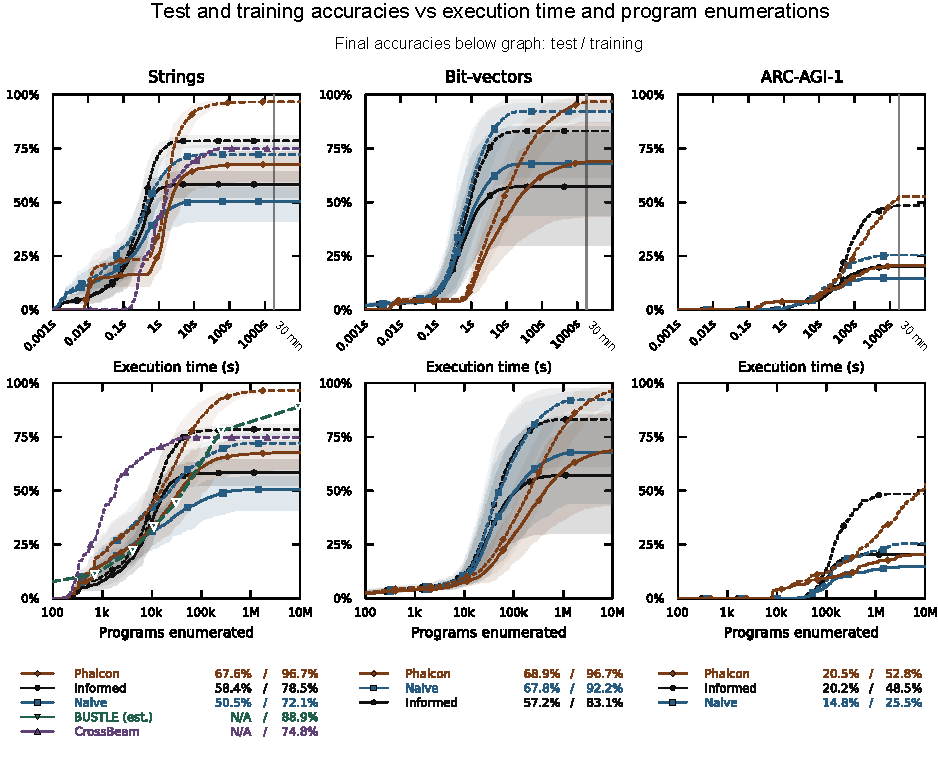
\includegraphics[width=0.8\textwidth]{figures/1-baseline-comparison.pdf}
  \caption{Comparison with baselines by execution time and program enumerations.}
  \label{fig:eval-heuristics}
\end{figure*}


\begin{figure*}[!t]
  \centering
  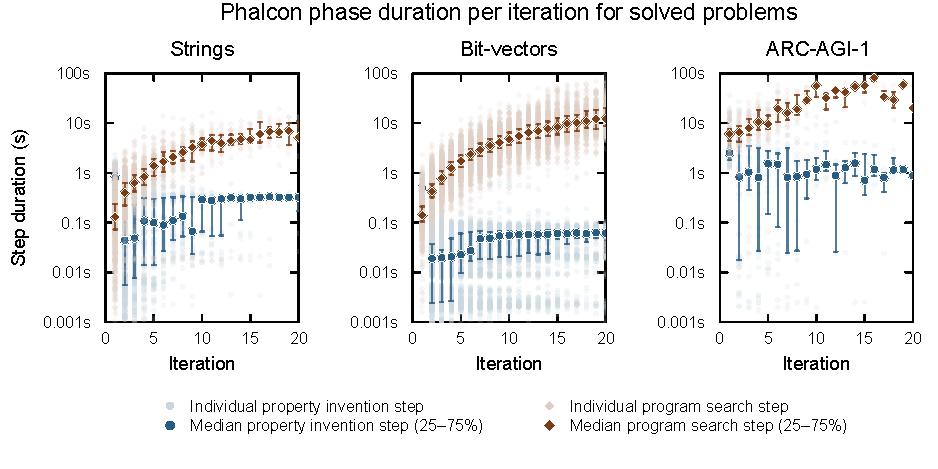
\includegraphics[width=0.8\textwidth]{figures/1a-phase-step-duration.pdf}
  \caption{Time spent in program search and property invention during PHALCON iterations.}
  \label{fig:eval-phase-time}
\end{figure*}

\subsection{Experiment 2: Agreement Threshold}
This variant relaxes PHALCON's preference for selective properties.
Recall that default PHALCON enumerates properties until it finds one
with agreement one. This variant stops at the first property whose
agreement count is positive and at most a given threshold. If no candidate
qualifies within the budget, it uses the property with the smallest
positive agreement count found. Raising the threshold can shorten
property search while making it easier for the current population to
satisfy the selected goal, but also making the property less informative
for guiding search. 
We compare thresholds of 1, 5, 10, 25, 50, and 99. We exclude a
threshold of 100 because it permits properties that agree with the
entire population, including constant properties such as
\(\pi(x,y)=(y=y)\).

The results can be seen in Figure~\ref{fig:eval-threshold}.
Performance is similar across agreement thresholds. At the extreme threshold of 99, execution time increases slightly,
but performance eventually converges.

PHALCON therefore appears to need a sufficiently informative property,
rather than the most selective property available.

\begin{figure*}[!t]
  \centering
  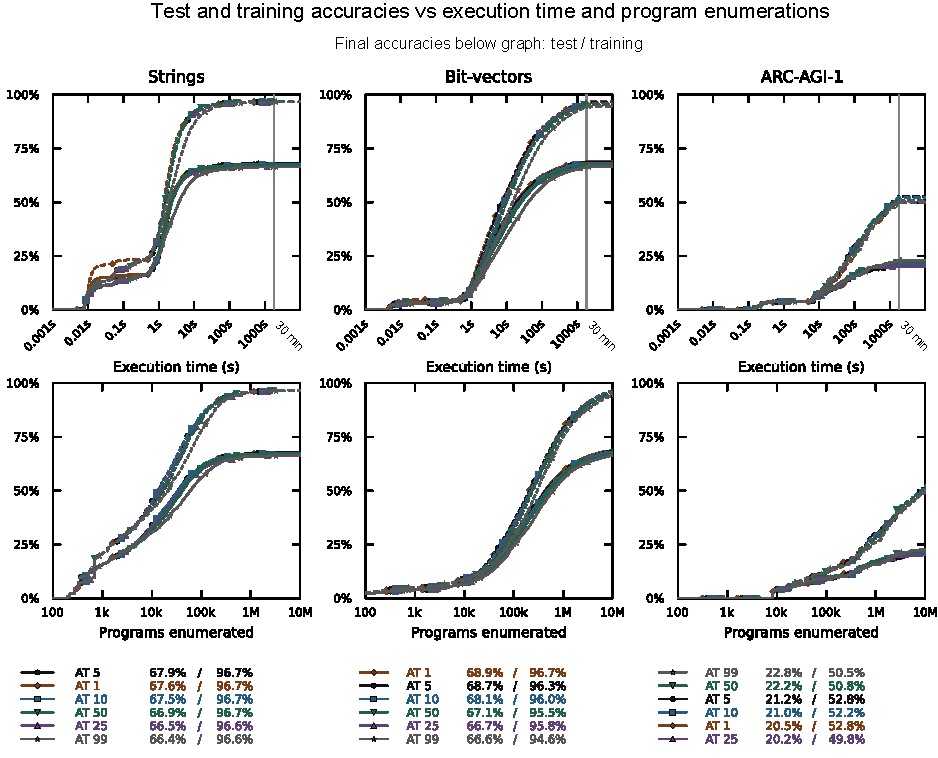
\includegraphics[width=0.8\textwidth]{figures/2-acceptance-threshold-comparison.pdf}
  \caption{Comparison of PHALCON agreement thresholds by execution time and program enumerations.}
  \label{fig:eval-threshold}
\end{figure*}

\subsection{Experiment 3: Batch Selection}
This variant removes the iterative property selection process of PHALCON.
It collects a single initial sample of distinct output vectors and ranks
candidate properties by their agreement on that sample. We prevent
selecting equivalent properties by ensuring that selected properties
agree with different subsets of the sampled outputs.
We experiment with batches of 5, 10, 20, or 40 properties and compare
them with default PHALCON. To give each batch the same number of outputs
per property as default PHALCON, we use sample targets of 500,
1,000, 2,000, or 4,000 distinct output vectors, respectively, giving
each batch 100 output samples per property.

Figure~\ref{fig:eval-batch} shows that selecting a single batch reduces
overall accuracy relative to iterative selection. Nevertheless, a batch
provides more guidance than a single property: it solves substantially
more problems than standard PHALCON reaches with zero or one selected
properties. This motivates selecting batches iteratively, but there is
a trade-off. Selecting several goals at once can reduce the number of
program searches, while evaluating more properties makes each candidate
program more expensive to score. A batch may also introduce more goals
than are needed.

To examine this trade-off, we compare batch size five with standard
PHALCON on shared solves (Figure~\ref{fig:eval-batch-shared}). We choose
the smallest batch to limit the additional work caused by additional
properties. Batch selection consistently reduces program enumerations,
but increases overall execution time. Thus, batching can reduce the
number of programs searched while increasing the cost of each evaluation.

\begin{figure*}[!t]
  \centering
  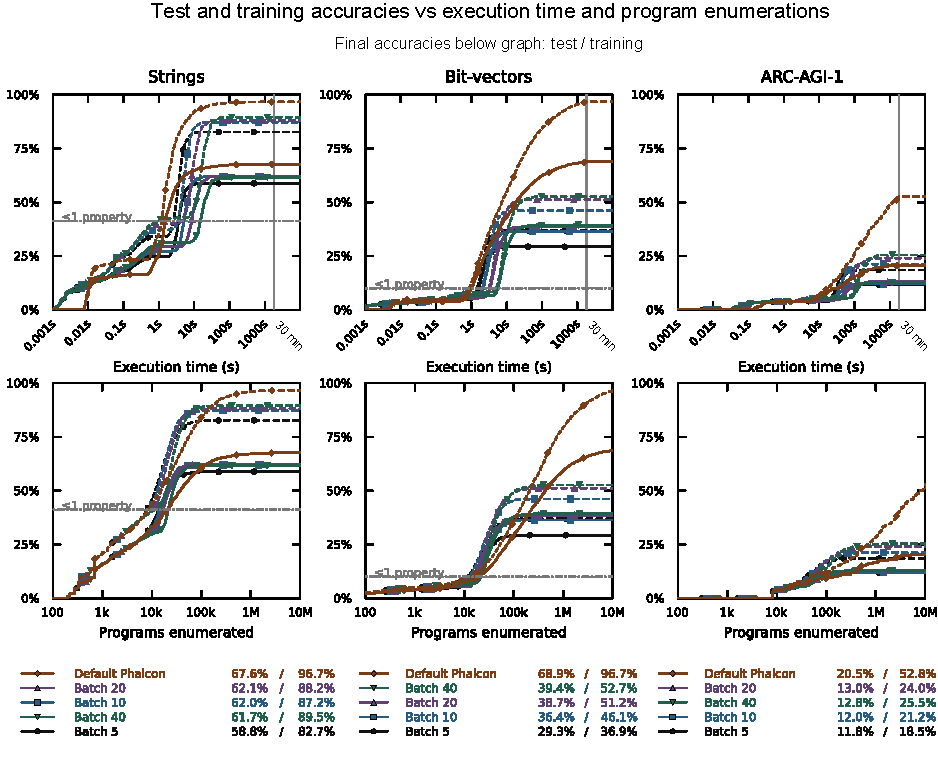
\includegraphics[width=0.8\textwidth]{figures/3-phalcon-batch-comparison.pdf}
  \caption{Comparison of batch selection with iterative PHALCON. Reference lines show the accuracy reached with at most one property.}
  \label{fig:eval-batch}
\end{figure*}


\begin{figure*}[!t]
  \centering
  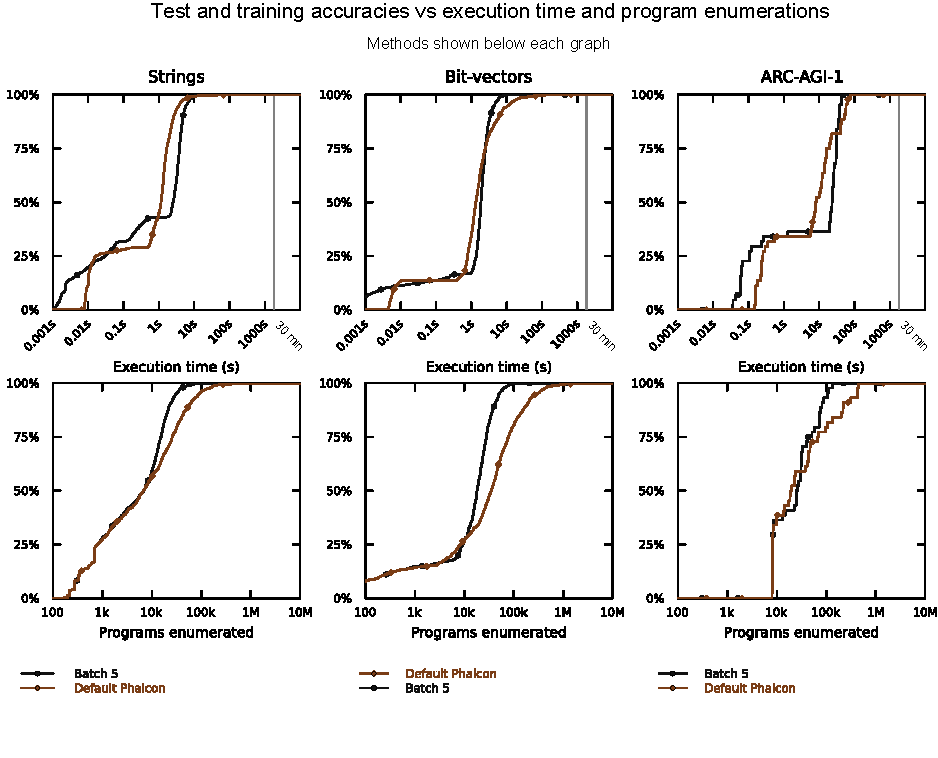
\includegraphics[width=0.8\textwidth]{figures/3a-batch5-shared-solves.pdf}
  \caption{Batch size five and standard PHALCON on shared solves.}
  \label{fig:eval-batch-shared}
\end{figure*}

\subsection{Experiment 4: Domain-Level Selection}
This variant removes task-specific property selection. It derives a
shared set of properties from sampled programs across the domain.
For each problem, we sample up to 100 distinct program output vectors
and rank candidate properties by agreement, preferring lower positive
agreement counts. We assign zero agreement a score of 100, giving it the worst possible
rank, tied with properties that agree with all 100 outputs. We combine these per-problem rankings using Friedman ranking:
tied scores receive average ranks, and properties are ordered by their
mean rank across problems. This yields a single domain-wide ranking.
We test the 5, 10, 20, or 40 best-ranked properties. Comparing this fixed set with PHALCON tests the
value of selecting properties for each task during search.

The string benchmark is a special case because its problems have
different input and output types. For this experiment, we restrict
the benchmark to the 67 problems with a single string input and a
string output.

% Finalize the domain-ranking protocol, comparison settings, and results.


Figure~\ref{fig:eval-domain} shows that using only properties selected
for the domain yields substantially lower accuracy than selecting
properties for each task. These results favor task-specific goals over
a fixed set of domain-specific goals.


\begin{figure*}[!t]
  \centering
  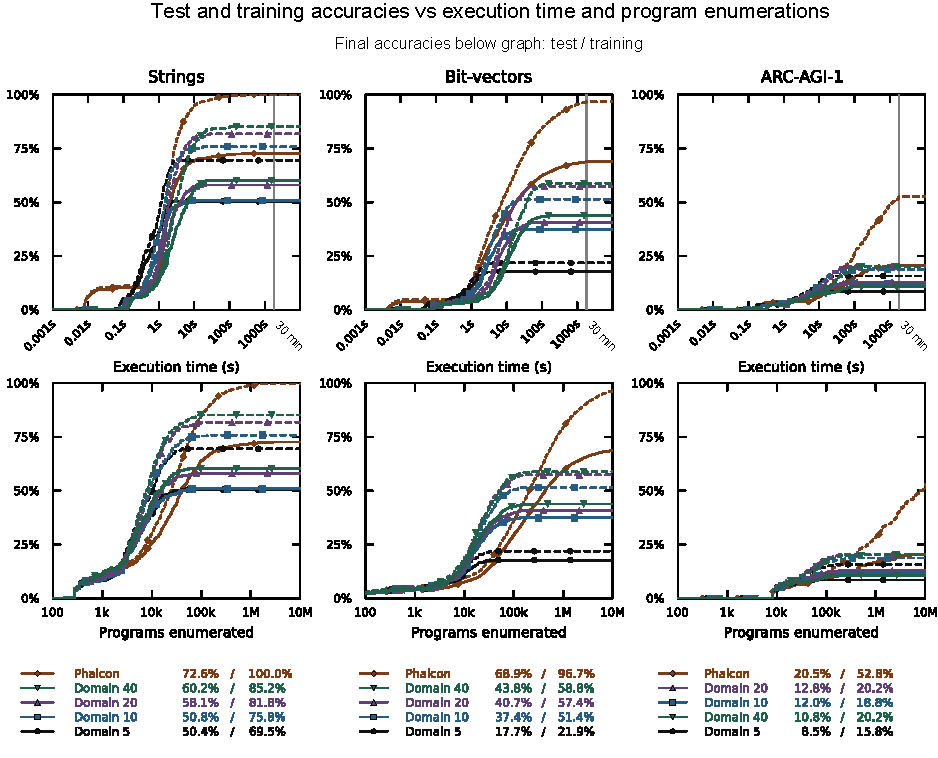
\includegraphics[width=0.8\textwidth]{figures/4-phalcon-domain-comparison.pdf}
  \caption{Comparison of domain-level property selection with task-specific PHALCON.}
  \label{fig:eval-domain}
\end{figure*}

\subsection{Ablation Study 1: Property Enumeration Cap}
A larger property enumeration cap increases the chance of finding a
property with agreement one, but also permits longer property searches.
We seek a cap beyond which further enumeration yields little improvement
in this success rate. We measure the candidates needed at each property
invention step for three problems from each domain, using populations
of 10, 25, 50, 100, 250, and 500 and a cap of 50,000 candidates per step.
Figure~\ref{fig:eval-budget} plots the percentage of invention steps
that find an agreement-one property against candidate evaluations.

The curves show that increasing the cap beyond 10,000 offers little
additional improvement. We therefore use 10,000 as the standard cap.


\begin{figure*}[!t]
  \centering
  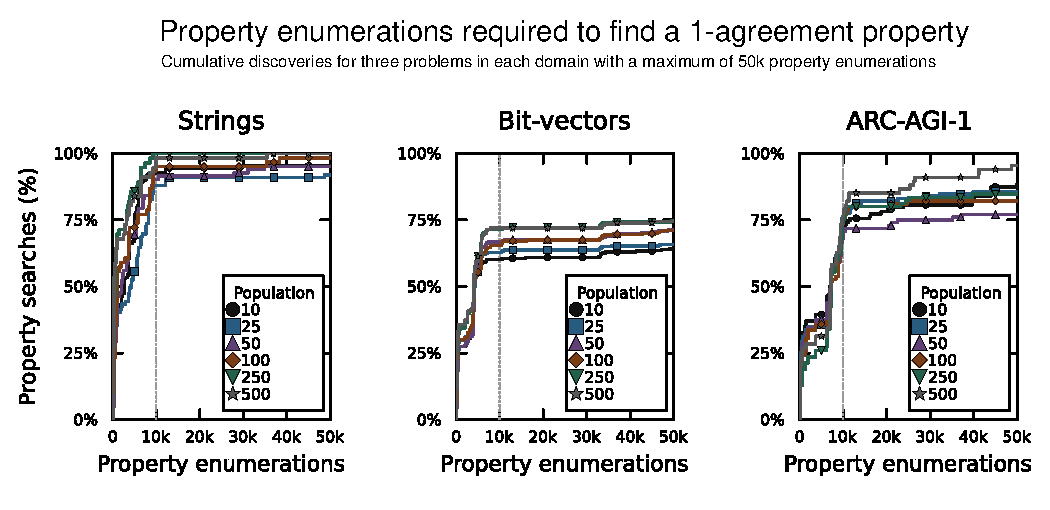
\includegraphics[width=0.8\textwidth]{figures/A.1-property-enumeration-cumulative.pdf}
  \caption{Percentage of property invention steps reaching agreement one as candidate evaluations increase, across population sizes and domains.}
  \label{fig:eval-budget}
\end{figure*}

\subsection{Ablation Study 2: Population Size}
Population size determines how many distinct program behaviors can
inform a property-selection round. A larger population can expose more
partial matches while requiring more work to construct and evaluate.
This ablation varies population size to assess that trade-off.
We compare populations of 10, 25, 50, 100, 250, and 500 under the
same per-iteration candidate cap.


Figure~\ref{fig:eval-population} shows similar trends across population
sizes in all three domains. Small populations reduce overall accuracy
on bit-vectors and ARC, while larger populations increase execution time
and program enumerations on strings. We choose a population of 100
because it is large enough to attain the observed accuracy while
limiting the additional search cost.


\begin{figure*}[!t]
  \centering
  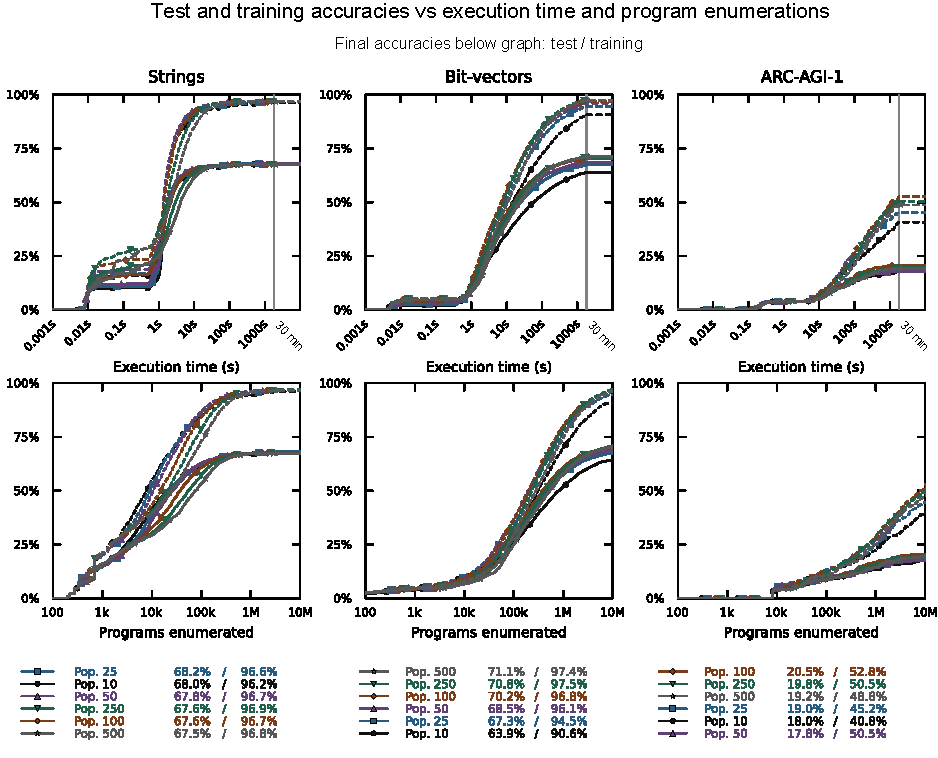
\includegraphics[width=0.8\textwidth]{figures/A.2-population-ablation.pdf}
  \caption{Population-size ablation by execution time and program enumerations.}
  \label{fig:eval-population}
\end{figure*}

% Prior-work leads for the scoped novelty claim:
% Probe: https://arxiv.org/abs/2010.08663
% FrAngel: https://arxiv.org/abs/1811.05175
\section{Related Work}
\label{sec:related-work}

Few methods closely resemble PHALCON's generation of goals during
search for an individual task. Related approaches typically rely on
pre-training across tasks or abstractions tailored to a domain.

\paragraph{Synthesis through Abstract Interpretation.}
Abstract interpretation summarizes program behavior through selected
properties \citep{cousot1977abstract}. In synthesis, these summaries can
eliminate families of programs whose abstract behavior conflicts with
the specification. Absynthe uses abstract interpretation to guide
top-down synthesis \citep{guria2023absynthe}, while iterative
forward--backward abstract interpretation combines information from
partial programs and candidate subexpressions \citep{yoon2023inductive}.
BLAZE refines abstractions to narrow an automaton representing candidate
programs \citep{wang2018abstraction}.

The effectiveness of this pruning depends on the abstraction and on
sound abstract semantics for the grammar's operations. Properties must
capture useful distinctions, and the abstract semantics must propagate
them precisely enough to reject incompatible candidates.

\paragraph{Learning Heuristics with Properties.}
Property signatures represent program behavior using a fixed collection
of Boolean properties \citep{odena2020signatures}. Each property is
evaluated across the examples and summarized according to whether it is
always true, always false, or mixed. These signatures describe tasks and
intermediate values for learned search heuristics. BUSTLE uses them to
prioritize subexpressions during bottom-up synthesis
\citep{odena2021bustle}. \textsc{CrossBeam} learns how to combine previously
generated expressions \citep{shi2022crossbeam}, and \textsc{LambdaBeam} extends
this approach to higher-order functions and lambda expressions
\citep{shi2023lambdabeam}.

\section{Discussion and Conclusion}
Our results support extracting partial goals from candidate programs as
a way to guide inductive program synthesis. PHALCON achieves accuracy
comparable to or higher than the evaluated baselines across the tested
domains. These results show that properties discovered during search
can capture useful progress towards satisfying the examples. However,
PHALCON requires more time to reach comparable accuracy. Almost all of
its execution time is spent in the relatively simple genetic programming
search used to satisfy the selected goals. Improving program search
under these goals is therefore a central direction for future work.

The agreement-threshold experiment also suggests that PHALCON's
preference for the most selective property found within its enumeration
budget can be relaxed. With a population of 100, accepting a property
that agrees with up to 50 programs gives performance similar to standard
PHALCON. A property can therefore provide useful guidance even when
many candidates already satisfy it. This opens the selection criterion
to considerations beyond selectivity. Future work could favor goals
that are easier to satisfy, whose satisfaction is more likely to survive
genetic mutations and crossover, or whose structure permits directly
constructing programs that satisfy them. Such criteria could connect
goal selection more closely to the capabilities of the program search.

The batch and domain-level experiments favor selecting goals for each
task and updating them as search progresses. Batches reduce program evaluations on shared solves but increase
execution time and solve fewer tasks. Shared domain properties also
reduce accuracy. These results show that useful goals depend on the
task and the current search state.

PHALCON also offers a practical advantage when moving between domains.
It requires no pre-training on synthesis tasks or prior learning of a
domain-specific search policy. Given input--output examples and suitable
program and property grammars, it generates its guidance during the
synthesis attempt itself. This makes the method applicable without a
training corpus or a separately trained model for the new domain.

% Any appendix included in this PDF counts toward the seven content pages.
% Place it before the bibliography. Optional technical supplements are separate PDFs.

\bibliography{references}

\end{document}
